%!TEX root = ../../csuthesis_main.tex
\chapter{绪论}



\section{研究背景}

随着人工智能、计算机视觉及自动控制等技术的迅猛发展,自动驾驶作为智能交通体系中的核心环节,正在从理论研究走向商业化落地。自动驾驶系统通常由感知、决策与控制三大模块构成,其中视觉感知作为信息获取的前端环节,其精度和稳定性直接影响整个系统的安全性与智能性。在复杂交通环境中,车辆与行人等动态目标的准确识别、持续跟踪以及行为意图的及时判断,是实现安全驾驶与合理路径规划的基础保障。

当前,基于深度学习的目标检测与多目标跟踪算法在学术界与工业界中得到广泛应用,其中以YOLO系列、SORT/DeepSORT等方法为代表的视觉跟踪算法已具备较高的实时性与鲁棒性。然而,在实际交通场景中,单纯的跟踪信息往往不足以支撑高级驾驶辅助功能(ADAS)的需求。系统不仅需要知道“是什么”和“在哪里”,更需要理解“它想要干什么”,即对前方目标的运动趋势与行为意图做出合理判断,从而提前进行风险预判与决策干预。这种基于时空轨迹与速度信息的意图识别能力,将成为未来智能驾驶系统的重要能力之一。

另一方面,受限于真实交通场景数据采集的高成本与不可控性,虚拟仿真平台在智能驾驶算法研发中发挥着重要作用。Carla作为目前最具代表性的自动驾驶开源仿真平台之一,提供了高度还原真实城市交通环境的三维场景与丰富的传感器模拟能力,为研究人员提供了可控、可复现的实验环境。本研究基于Carla平台,通过构建可运行的目标跟踪与意图识别系统,完成视觉感知到智能判断的全流程设计与实现,具有重要的研究价值和现实意义。

综上所述,开展面向自动驾驶的视觉目标跟踪与意图分析研究,既能够推动感知系统从“感知当前”向“预测未来”的进化,也有助于提高自动驾驶系统的安全冗余能力和交通行为的合理性。本课题的研究成果可为未来多目标智能预测、复杂场景理解等方向提供工程实践基础与技术参考,具有良好的应用前景。

\section{国内外研究现状}

\subsection{目标检测研究现状}

目标检测是指将图像或者视频中的目标与其他不感兴趣区域进行区分,判断是否存在目标,以及确定目标位置和识别目标种类的计算机视觉任务。以是否使用深度学习为分界线,可以将目标检测算法分为传统的目标检测算法和基于深度学习的目标检测算法。传统的目标检测算法依赖于人工设计的特征算子,并采用特征提取加分类器的模式来实现。Viola和Jones提出了Viola-Jones人脸检测器 \cite{viola2001rapid},该检测器使用Haar-like特征提取算子,利用Adaboost分类器进行分类,并采用由多个分类器组成的Cascade级联分类器来提高识别率。Navneet Dalal等人\cite{dalal2005histograms}提出方向梯度直方图(Histogram of Oriented Gradients,HOG),HOG是一种用于目标检测的特征描述算子,通过计算图像中局部梯度的方向信息,对图像的浅层外观特征进行提取。由于HOG过度依赖局部梯度信息,因此在复杂场景下的特征提取能力较差。Felzenszwalb等人\cite{felzenszwalb2009object}在HOG的基础上,提出了可变形组件模组(Deformable Part Model,DPM)。DPM采用多组件策略,将目标分解为多个部分后进行建模,因此DPM对目标的形变具有很强的鲁棒性。传统的目标检测算法大多使用人工设置的特征提取算子来对图像进行特征提取,在面对多尺度、密集目标、极端天气等复杂环境时,算法的鲁棒性和准确率都会大大降低。同时采用滑动窗口来对图像特征进行逐一计算的方式,会使算法的计算复杂度过高。因此传统的目标检测方法无法满足实时检测需求,不能很好地在工业中进行应用。

随着深度学习的飞速发展,目标检测领域的研究取得了突破性的进展。与传统的目标检测算法相比,基于深度学习的目标检测模型在经过大量图像数据训练后,能“学会”如何提取目标特征,在面对不同尺度的目标以及复杂场景时,具有更好的鲁棒性和泛化能力。根据是否需要生成候选区域,可以将基于深度学习的目标检测算法分为单阶段(one-stage)与两阶段(two-stage)。两阶段的目标检测算法主要分为两步,首先筛选出图片中可能包含物体的候选区域,接着再对候选区域中的特征进行分类回归。Ross Girshick等人\cite{girshick2014rich}提出R-CNN目标检测算法,首先对输入图像使用选择搜索\cite{uijlings2013selective}(selective search)网络获得大约2000个不同尺度的候选区域,接着对所有的候选区域进行统一缩放,将尺寸变为227×227。再通过卷积神经网络(Convolutional Neural Networks,CNN)对所有候选区域中的特征进行提取,得到维度为2000×4096的特征向量。最后再利用SVM分类器对特征向量进行分类,以及使用回归器来对边界框的位置进行调整。由于R-CNN目标检测算法需要对约2000个候选框逐一进行特征提取,而候选框之间又存在许多包含相同特征的区域,这就导致整个过程中存在大量冗余操作,严重影响了检测速度。为了解决上述问题,Ross Girshick等人\cite{girshick2015fast}又提出了Fast R-CNN,Fast R-CNN首先对输入的图像进行卷积,得到对应的特征图。接着将事先处理好的区域候选框投影到特征图上。采用这种方式只需要进行一次卷积,可以减少大量冗余的卷积计算。而且与R-CNN所使用的分类任务+回归任务模式不同,Fast R-CNN将二者融合在一个网络中,不再需要对分类器和回归器进行单独训练。但是Fast R-CNN算法依然沿用了使用选择搜索算法的方式来获取候选区域,该过程不仅操作耗时而且容易漏掉包含目标的区域。因此Shaoqing Ren等人\cite{ren2015faster}又提出了Faster R-CNN,算法采用区域建议网络(Region Proposal Networks,RPN)来获取区域候选框,实现了生成候选区域过程与目标检测任务的融合。同时Faster R-CNN还提出了锚框(Anchor)这一重要思想,锚框是指在图像上预先设置好多组尺寸比例不同的参照框,来尽可能地包含物体出现的位置。He Kaiming\cite{he2017mask}等人在Faster R-CNN的基础上提出了Mask R-CNN,该算法使用ROIAlign替换Faster R-CNN中的ROIPooling。ROIAlign可以将任意尺寸感兴趣区域的特征图划分为具有固定尺寸的小特征图,并使用双线性插值取代了ROIPooling中的直接取整操作,解决了ROIPooling操作中因两次量化造成的区域不匹配(mis-alignment)问题。在目标检测任务中,使用IOU阈值来区分正负样本。当IOU阈值越大,正样本的数量就会减少,而减小IOU阈值又会学习到大量无关特征。Cai等人cite{cai2018cascade}为了解决上述问题,提出了Cascade R-CNN,该算法采用级联式的结构,通过对多个感知器使用递增的IOU阈值进行训练,来解决因提高IOU阈值所引起的模型过拟合问题。

\subsection{目标跟踪研究现状}

多目标跟踪算法可以分为基于检测跟踪(Tracking by Detection, TBD)和联合检测跟踪(Joint Detecting Tracking, JDT)两种方式。TBD 目标跟踪算法是指先使用目标检测算法得到包含物体的边界框,接着再获取目标的运动信息和外观信息等,最后通过数据关联算法来计算目标间的亲和力并关联目标。Bewley等人\cite{bewley2016simple}提出了 SORT 算法,作为经典的基于检测的目标跟踪算法,采用 Faster R-CNN 作为检测器,利用卡尔曼滤波来预测和更新物体的运动特征信息,通过匈牙利算法进行数据关联,以及使用 IOU 作为度量指标来建立关系,从而实现对多目标进行追踪。Wojke 等人\cite{wojke2017simple}提出了 DeepSORT 多目标跟踪算法,该算法在 SORT 的基础上加入级联匹配,引入了卷积神经网络来提取目标外观特征,有效地减少了在面对遮挡情况下发生身份切换的问题。Yu 等人\cite{yu2016poi}提出了 POI 算法,采用 Faster R-CNN 作为检测器,并使用 skip pooling 和 multi-region 两种策略来提高检测精度,利用改进的 GoogLeNet\cite{szegedy2015going}网络进行特征提取。Sun 等人\cite{sun2019deep}提出了深度亲和网络(DAN),DAN 网络以端到端的方式对目标物体的外观特征进行学习,通过物体和环境的分层特征计算出在不同帧中目标之间的亲和度。Chen 等人\cite{chen2018real}将检测和跟踪结果组成一对候选框,提出了一种得分函数用于衡量每一对候选框的匹配程度,使用非极大值抑制算法依据得分情况进行筛选。Zhang 等人\cite{zhang2021fairmot}将目标检测任务和特征提取融合到一个网络中完成。首先使用编码器-解码器模块对图像进行特征提取,在进行分流后,使用两个分支分别进行边界框预测以及目标外观特征提取,最后使用预测目标中心点处的特征进行边界框时序联结。Liang 等人\cite{liang2022rethinking}提出 CSTrack 算法,采用 CCN(交叉相关网络)来改进检测与重识别间的协作学习。将目标检测和外观特征提取进行解耦,通过使用自注意力的方式获得自注意力权重图和交叉相关性权重图,并利用 SAAN\cite{zhao2020saan}(尺度感知注意力网络)对特征提取网络进行优化。Liang 等人\cite{liang2022fake}在 CSTrack 的基础上引入时间信息来修正检测器结果,并提出了重检测网络来重新加载被错误分类的目标。Yu 等人\cite{yu2022relationtrack}提出了 GCD(Global Context Disentangling)模块,该模块能将特征图解耦成检测特征和重识别特征两部分,同时采用可变形注意力机制来学习目标和环境之间的关系。

联合检测跟踪算法是将检测任务与跟踪任务进行合并,仅使用一个网络来实现多目标跟踪任务。Peng 等人\cite{peng2020chained}提出了一种 CTracker 算法,该算法首次将目标检测、特征提取、数据关联三个模块集成到单个网络中,实现了端到端的联合检测跟踪。同时还设计了一种联合注意力模块(JAM,Joint Attention Module)来突出检测框中的有效信息区域。Xu 等人\cite{xu2020deep}提出了 DHN(深度匈牙利算法),以可微的方式对检测框和预测框进行匹配,以及提出了一种新的损失函数用于训练联合检测跟踪范式的多目标跟踪器。Pang 等人\cite{pang2021quasidense}提出 QDTrack 算法,通过采用多个正负样本同时计算损失的方式来对特征提取网络进行训练,是一种只利用 ReID 特征而不需要位置和运动信息的多目标跟踪方法。Zhou 等人\cite{zhou2020tracking}提出了 CenterTrack 算法,使用 CenterNet\cite{zhou2019objects}目标检测算法来对目标中心进行定位,CenterTrack 依据上一帧的检测结果得到热量图,峰值代表目标中心点,并采用高斯渲染的方法进行模糊处理。模型利用两个额外的并行分支来预测当前目标相对于上一帧时的水平和竖直方向偏移量。Wu 等人\cite{wu2021track}提出了一种在线多目标联合检测追踪模型,使用 CenterNet 提取图像特征,利用 CVA 模块计算两帧图像中目标的偏移量,得到目标之间的关联性,通过 MFW 模块来传播和增强目标特征,最后使用头部网络将传播特征和当前特征进行处理以实现检测和追踪。Wang 等人\cite{wang2021multiple}提出了 CorrTracker 算法,利用局部相关模块来构建目标与周围环境之间的拓扑关系,从而加强模型在密集场景中的识别能力。Sun 等人\cite{sun2020transtrack}提出 TransTrack 算法,该算法采用 transformer\cite{vaswani2017attention}架构,利用 Query-Key 机制来跟踪当前帧中已存在的目标以及对新目标进行检测。通过在一次拍摄中完成目标检测和目标关联,建立了一种新的联合检测跟踪范式。Chu 等人\cite{chu2023transmot}提出了 STGT 模型,通过将追踪目标轨迹视作稀疏赋权图来构建目标间的空间关系。STGT 构建了一个空间图 transformer 编码器、时间 transformer 编码器和一个空间 transformer 解码器。利用稀疏图来提升训练和推理时的计算速度。并且由于获取了目标间的结构信息,因此比一般的 transformer 也更加有效。

\subsection{意图分析研究现状}

最早关于识别驾驶意图的讨论可以追溯到 Andrew 等人的一项研究\cite{liu1997realtime},他们认为可以通过分析驾驶员的行为动作来预测其意图,并在研究中仅使用车辆的动态数据,例如横摆角、横摆角速度和车速,来判断驾驶员是否有转弯或换道的意图。要对周围车辆的换道意图进行识别,需要结合感知、数据融合、数据处理等多种技术\cite{zhang2023highway}。感知与数据融合技术融合所有从传感设备传输的信号,生成周围所有交通和其他环境的信息。智能车辆将这些信息从自身的车辆坐标系转换为目标车辆坐标系,并处理为识别算法可以使用的特征变量。因此,在识别方法之外,特征变量的选择对识别的效果也影响重大。针对单个目标车辆,目前广泛使用的信号包括纵向/横向位置、速度和加速度\cite{woo2017lane}。主车的意图识别可以通过车内传感器获得大量有效信息,比如方向盘和制动/油门踏板信号,甚至驾驶员本身的状态等。然而,在车联网技术尚未成熟的当下,目标车辆内的这些信息难以获取。Zhang 等\cite{zhang2018lane}使用目标车辆及其四辆邻近交通车辆的信息,包括它们之间的相对速度和距离,来预测换道行为。Leonhardt 等\cite{leonhardt2017feature}也采用了类似的特征变量来研究换道预测。部分研究使用了目标车辆周围的更多相邻车辆以及与每个相邻车辆相关的更多信息(比如状态量的历史记录)\cite{patel2018predicting}。Altch 等\cite{altche2017lstm}甚至考虑了九辆车来提高预测性能。

2016 年,日产研制出了前沿科技 ProPILOT,其安装的实力强劲的摄像机可以较为容易的检测出车相对道路的偏离距离\cite{zhang2016nissan}。雪铁龙 LDWS 系统安装有 6 个电子传感器。汽车通过车道标记线的时候,光线的反射不一样,此时检测单元会将信息发送到车载控制中心,内置的振动马达会向驾驶员传递警告信息。这个系统的价格低廉,系统的适应性不错,但是在复杂的电子环境下的表现会受到影响,元器件的精度会降低,目前在 C5、C6 的车型上有应用。Google 也进行了相关研发,利用高性能的软件和智能探测装置,融合雷达和摄像技术,能够在复杂条件下全面的探测周围环境\cite{wang2020autonomous},其结合 GPS 技术的车道偏离技术可以及时矫正汽车的行驶轨迹,并且误差可以达到厘米级。Enache 等\cite{enache2009driver}提出了新的计算方法,通过预瞄偏差及车辆方向偏差综合信息来估计车路之间的相对距离;Cualain 等\cite{cualain2012automotive}利用卡尔曼滤波和霍夫变换建立了车道边界的模型,计算车辆本身的参数及建立新的预警规范来设计预警系统的阈值;Mammar 等cite{mammar2006time}通过计算道路曲率、方向偏差等估计车辆跨过车道线的时间;Ulsoy 等\cite{chiu1996time}利用准确度较高的算法估计TLC 的不确定,考虑到了不同方面的误差;Gaikwad 等\cite{gaikwad2015lane}通过对感兴趣区域的划分,建立实际车道偏离的度量标准。

\section{研究目标与内容}

本课题旨在设计并实现一套基于视觉感知的自动驾驶目标跟踪与意图分析系统,借助 Carla 仿真平台构建可控的交通环境,通过集成深度学习目标跟踪算法和基于物理信息的行为推理机制,实现对动态交通目标(如车辆、行人)的连续识别、轨迹跟踪与运动意图判断,并能够在图形界面中实时可视化跟踪过程与分析结果,从而为智能驾驶系统提供基础性的感知支撑。

为实现上述目标,本课题主要围绕以下几个方面开展具体研究与开发工作:

\textbf{数据集构建与处理。}在 Carla 提供的仿真场景中,部署本车及自动生成车流,通过挂载 RGB 摄像头对周围交通目标进行图像采集与注释,提取包含图像帧、目标边界框、目标速度等信息的原始数据,构建用于视觉分析的多模态数据集。同时,设计适用于后续分析与训练的统一标注格式和存储结构。

\textbf{视觉目标跟踪模型设计与集成。}本系统采用深度外观特征辅助的 DeepSORT 算法作为目标跟踪模型,通过对视频帧中的检测结果进行轨迹级别的数据关联,实现对车辆与行人的唯一身份标记与跨帧追踪。系统支持在单目标跟踪模式下自动选取“最接近本车”的目标进行持续跟踪,并将结果实时渲染在屏幕图像中。

\textbf{基于速度信息的意图分析方法设计。}在目标跟踪的基础上,提取目标在世界坐标系下的运动方向与速度大小,并结合其与本车的相对位置关系,设计运动意图识别规则体系。采用物理特征量(如点积关系、欧氏距离变化、速度阈值)判断目标是否存在“靠近”“远离”“危险靠近”等行为状态,并输出中文提示文本以实现可视化展示与预警反馈。

\textbf{系统集成与仿真测试。}将上述模块集成为一个完整的自动驾驶视觉分析系统,结合 Carla 提供的控制接口与传感器 API 实现全过程联动,在 Town10 与 Town01 两个典型城市街景场景中分别进行系统测试与功能验证,评估模型在不同场景下的运行效率与判断准确率,并结合帧率等性能指标进行可行性分析。

本研究面向自动驾驶核心任务需求,通过仿真数据采集、视觉跟踪、行为分析与实时展示四个维度开展工作,形成从感知到判断的完整流程,具备较强的应用价值与实践意义。

\section{本文结构框架}

本课题围绕自动驾驶场景下的视觉感知与行为预测展开,依托 Carla 仿真平台提供的高真实度交通环境与 Python 接口能力,采用模块化设计思路,构建了“数据采集—目标跟踪—意图分析—可视化展示”一体化流程,实现了一个可运行、可扩展的目标感知与行为识别系统。研究方法分为数据采集与预处理、目标跟踪算法设计、意图分析模块开发、可视化与系统集成四个主要环节,其整体流程如图所示:
\begin{figure}[H]
    \centering
    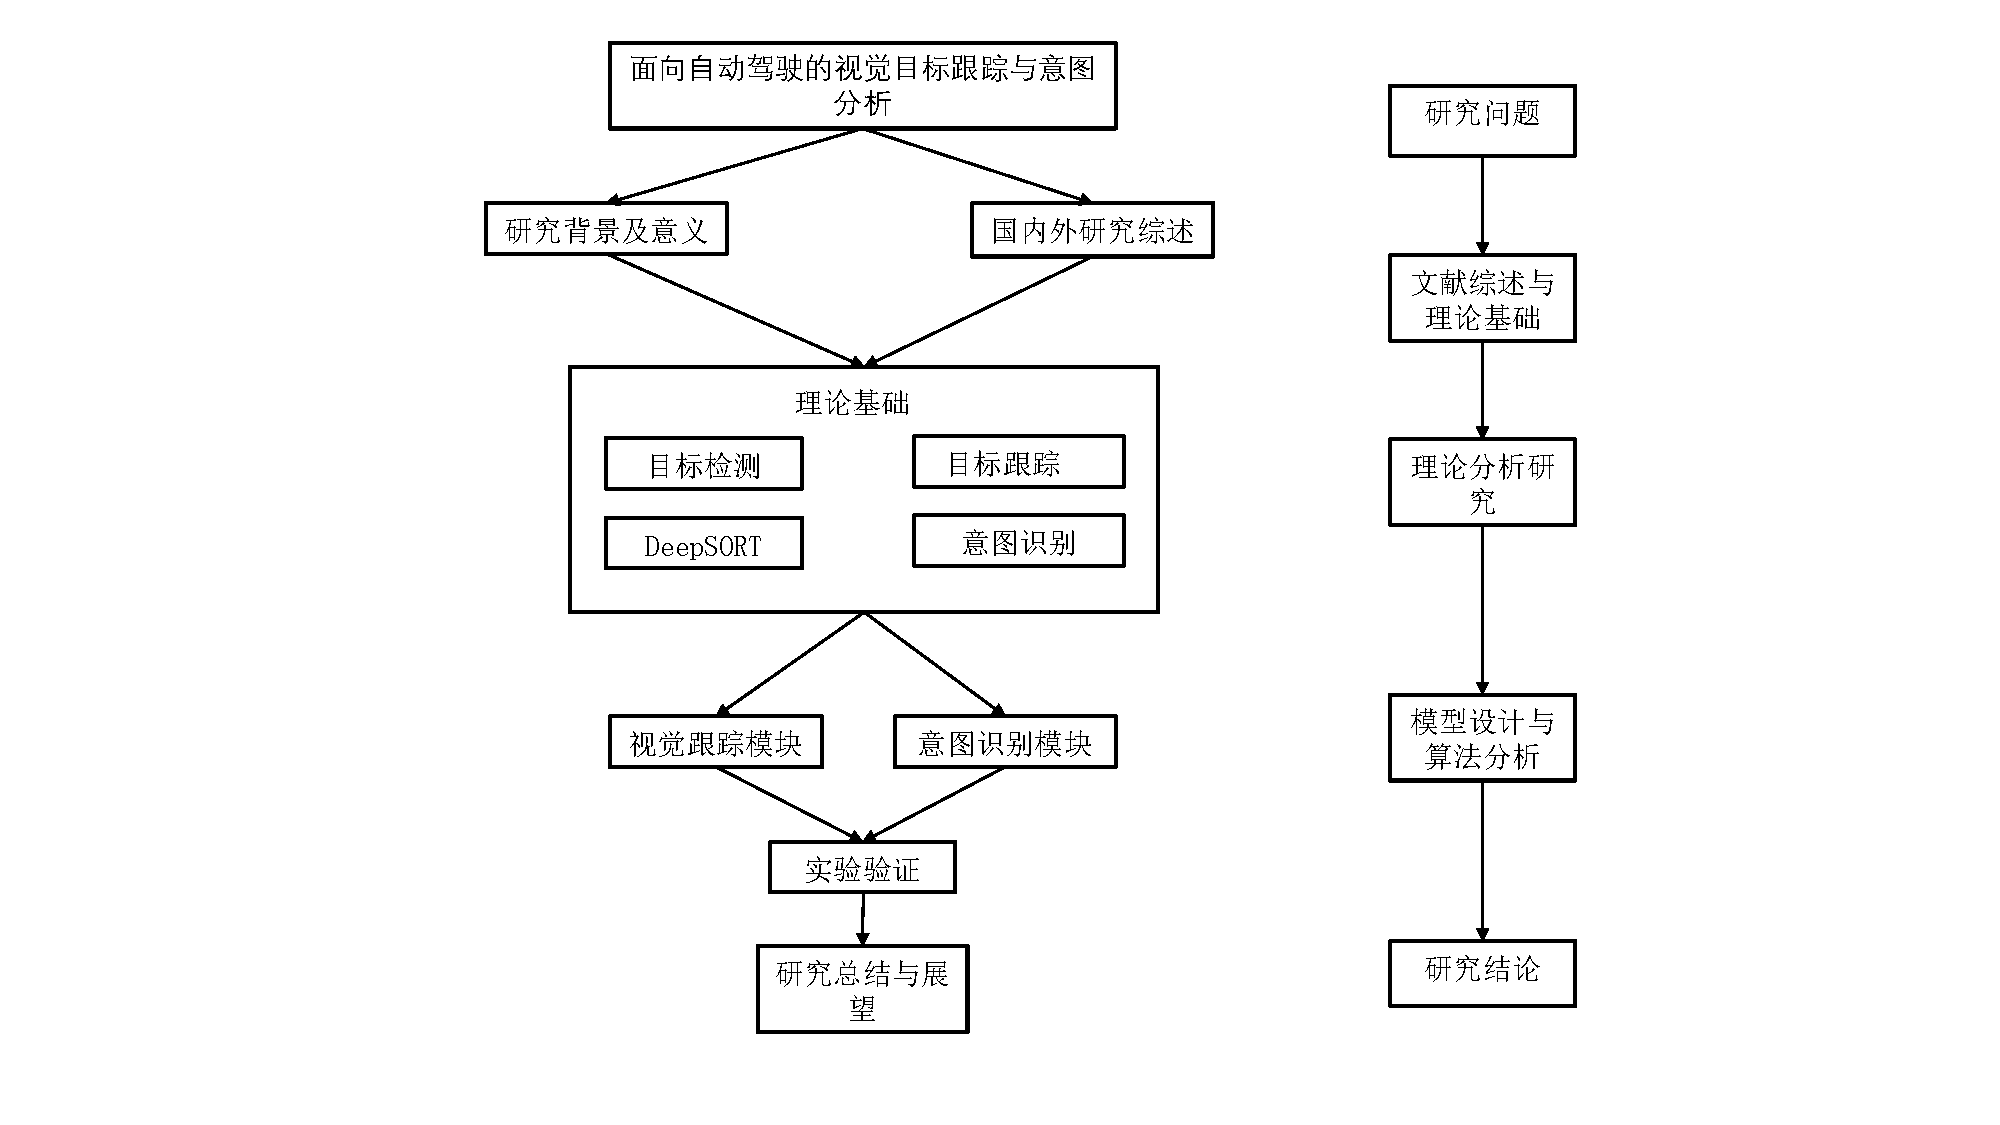
\includegraphics[width=0.8\textwidth]{images/图1 系统技术路线图.pdf}  % 引用转换后的 PDF 文件
    \caption{论文结构框架图}
    \label{fig:example_image}  % 可用于引用此图片
\end{figure}

在数据采集部分,系统通过 Carla 平台生成典型交通场景,优先选取 Town10 和 Town01 作为实验场地,并在本车上安装前向 RGB 摄像头以获取图像数据。每一帧图像经处理后可提取出车辆的二维边界框、目标ID、速度大小等结构化信息。为了实现后续训练与分析,系统在运行时自动保存图像帧(.jpg)和对应标注文件(.json),内容包括边界框坐标、目标速度、是否为当前跟踪对象等关键信息,构建出具备时序特征的感知数据集,确保可复现性和可扩展性。

目标跟踪模块是系统的核心部分。本设计集成了 DeepSORT 跟踪算法,其结合了外观特征提取与卡尔曼滤波器,在保持实时性的同时具备较强的数据关联能力。通过调用 Carla API,系统可实时获取当前场景中所有车辆的三维位置,并结合前端图像中的二维边界框,实现目标在图像空间内的连续标识。为保证算法聚焦于当前对本车最具潜在交互风险的目标,系统采用“最近目标优先”策略进行目标选择,并仅跟踪单个目标,从而有效降低计算开销并简化意图分析流程。

在行为识别方面,系统基于目标的速度向量、方向角度以及其与本车的相对位置,构建了轻量级的意图分析模块。该模块通过计算目标车辆的速度方向与本车之间的点积关系,结合速度大小与空间距离的动态变化,判断其当前行为趋势。具体包括“靠近中”“远离中”“危险靠近”“目标稳定”等状态,并通过阈值组合判断进行分级判断。在实际运行中,系统可实现对目标行为的实时预测,并将分析结果以中文文本的方式展示在跟踪框上方,增强系统的人机交互性和直观性。

整个系统的主控逻辑集中在 Carla 的同步刷新机制中,通过 game\_loop() 主循环完成数据获取、图像渲染、目标识别、意图计算与结果展示等全过程联动。系统采用 Pygame 进行图像渲染与键盘交互,支持用户手动操控本车行驶,同时自动完成图像与标签的保存工作,便于后续模型训练与性能评估。整体架构充分体现了模块化、可测试与可扩展的设计思想,能够有效支持不同场景下的视觉感知与行为分析研究,具有良好的工程实现基础。




\begin{tabular}{l l}
%  \verb|\songti| & {\songti 宋体} \\
%  \verb|\heiti| & {\heiti 黑体} \\
%   \verb|\kaiti| & {\kaiti 楷体}
\end{tabular}
